\documentclass[11pt,a4paper]{article}
\usepackage[utf8]{inputenc}
\usepackage[T1]{fontenc}
\usepackage{mathpazo}
\usepackage[scaled=0.92]{helvet}
\usepackage{courier}
\usepackage[a4paper,top=2.6cm,bottom=2.6cm,left=2.5cm,right=2.5cm,headheight=14pt]{geometry}
\usepackage{amsmath,amssymb}
\usepackage{xcolor}
\usepackage{graphicx}
\usepackage{tikz}
\usetikzlibrary{arrows.meta,positioning,calc,angles,quotes}
\usepackage{titlesec,fancyhdr,lastpage,booktabs,tabularx,enumitem,microtype,float,array,needspace}
\usepackage{caption}
\usepackage{subcaption}
\usepackage[colorlinks=true,linkcolor=azul,urlcolor=azul]{hyperref}

\definecolor{azul}{HTML}{1F3A5F}
\definecolor{azulclaro}{HTML}{E8EEF5}

% Sin patrones de separación silábica en español en este entorno: se evita partir palabras
\hyphenpenalty=10000 \exhyphenpenalty=10000 \emergencystretch=3em \tolerance=2000
\renewcommand{\contentsname}{Índice}
\renewcommand{\tablename}{Tabla}
\renewcommand{\figurename}{Figura}
\captionsetup{font=small,labelfont={bf,color=azul},labelsep=period}
\captionsetup[sub]{font=small,labelfont={bf}}

\titleformat{\section}{\needspace{6\baselineskip}\sffamily\Large\bfseries\color{azul}}{\thesection.}{0.6em}{}[\vspace{-4pt}{\color{azul}\rule{\linewidth}{0.6pt}}]
\titleformat{\subsection}{\needspace{4\baselineskip}\sffamily\large\bfseries\color{azul}}{\thesubsection}{0.6em}{}
\titlespacing*{\section}{0pt}{22pt}{8pt}
\titlespacing*{\subsection}{0pt}{12pt}{4pt}

\pagestyle{fancy}
\fancyhf{}
\fancyhead[L]{\sffamily\small GPS de Madrid: cálculo de rutas sobre grafos}
\fancyhead[R]{\sffamily\small Matemática Discreta · Práctica 3}
\fancyfoot[C]{\sffamily\small Página \thepage\ de \pageref{LastPage}}
\renewcommand{\headrulewidth}{0.4pt}

\setlength{\parindent}{0pt}
\setlength{\parskip}{6pt}
\setlist{itemsep=2pt,topsep=4pt}
\newcommand{\code}[1]{\texttt{#1}}

\begin{document}

% ---------------- Portada ----------------
\begin{titlepage}
\sffamily
\vspace*{1.5cm}
{\large Universidad Pontificia Comillas · ICAI\\[2pt]
Grado en Ingeniería Matemática e Inteligencia Artificial}

\vspace{3.2cm}
{\color{azul}\rule{\linewidth}{1.2pt}}\\[14pt]
{\fontsize{28}{34}\selectfont\bfseries\color{azul} GPS de Madrid}\\[8pt]
{\Large Cálculo de rutas sobre el grafo de calles de la ciudad}\\[10pt]
{\color{azul}\rule{\linewidth}{1.2pt}}

\vspace{1cm}
{\large Memoria técnica · Práctica 3 de Matemática Discreta}

\vfill
\begin{tabularx}{\linewidth}{@{}lX@{}}
\textbf{Grupo} & GP11B\\[3pt]
\textbf{Integrantes} & Jaime Tuesta de Simón\\
 & Ignacio Mascarell Agúndez\\[3pt]
\textbf{Asignatura} & Matemática Discreta (2.º curso)\\[3pt]
\textbf{Fecha} & Noviembre de 2025\\
\end{tabularx}
\vspace{1cm}
\end{titlepage}

\tableofcontents
\clearpage

% ---------------- 1 ----------------
\section{Introducción}

Este documento describe y justifica el procedimiento seguido para resolver la Práctica 3 de la asignatura de Matemática Discreta: el desarrollo de un sistema de navegación (GPS) para la ciudad de Madrid. El programa recibe una dirección de origen y otra de destino, calcula la ruta óptima entre ambas según el criterio elegido por el usuario y la presenta mediante instrucciones de navegación y un mapa con el recorrido resaltado.

La solución modela la red viaria como un grafo dirigido y pesado, en el que los nodos representan intersecciones y extremos de calle, y las aristas, los tramos que los unen. Sobre este grafo se aplica el algoritmo de Dijkstra con tres funciones de peso distintas: la longitud del tramo, su tiempo de recorrido y ese mismo tiempo más una penalización por semáforos.

A lo largo de la memoria se utiliza como ejemplo una ruta que cruza la ciudad de norte a sur, desde el Paseo de la Castellana, 144 (junto al estadio Santiago Bernabéu) hasta el Paseo de la Chopera, 14 (Matadero Madrid). Todas las figuras de mapas y de consola proceden de ejecuciones reales del programa.

% ---------------- 2 ----------------
\section{Arquitectura del programa}

El proyecto se organiza en cuatro módulos de Python con responsabilidades diferenciadas, que se resumen en la Tabla~\ref{tab:modulos}. La Figura~\ref{fig:flujo} muestra cómo fluyen los datos entre ellos para resolver una consulta.

\begin{table}[H]
\centering
\caption{Módulos del programa y responsabilidades.}\label{tab:modulos}
\small
\begin{tabularx}{\linewidth}{@{}lX@{}}
\toprule
\textbf{Módulo} & \textbf{Responsabilidad}\\
\midrule
\code{callejero.py} & Lectura y tratamiento del callejero de Madrid, búsqueda de direcciones (exacta y aproximada) y obtención del grafo de calles.\\
\code{gps.py} & Programa principal: interacción con el usuario, cálculo de la ruta, instrucciones de navegación y representación gráfica.\\
\code{grafo\_pesado.py} & Biblioteca de algoritmos sobre grafos pesados: Dijkstra, reconstrucción del camino mínimo, Prim y Kruskal.\\
\code{pesos.py} & Funciones de peso de las aristas: longitud, tiempo de recorrido y tiempo con semáforos.\\
\bottomrule
\end{tabularx}
\end{table}

\begin{figure}[H]
\centering
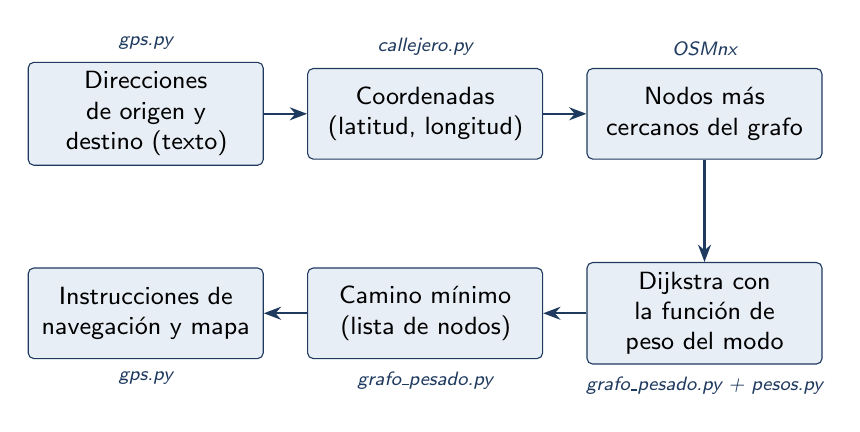
\begin{tikzpicture}[
  caja/.style={draw=azul,fill=azulclaro,rounded corners=2pt,align=center,font=\sffamily\small,minimum height=1.15cm,text width=2.75cm},
  modulo/.style={font=\sffamily\scriptsize\itshape,text=azul},
  flecha/.style={-{Stealth[length=2.2mm]},thick,azul},
  node distance=0.55cm and 0.55cm]
\node[caja] (dir) {Direcciones de origen y destino (texto)};
\node[caja,right=of dir] (coord) {Coordenadas (latitud, longitud)};
\node[caja,right=of coord] (nodos) {Nodos más cercanos del grafo};
\node[caja,below=1.3cm of nodos] (dijk) {Dijkstra con la función de peso del modo};
\node[caja,left=of dijk] (camino) {Camino mínimo (lista de nodos)};
\node[caja,left=of camino] (salida) {Instrucciones de navegación y mapa};
\draw[flecha] (dir) -- (coord);
\draw[flecha] (coord) -- (nodos);
\draw[flecha] (nodos) -- (dijk);
\draw[flecha] (dijk) -- (camino);
\draw[flecha] (camino) -- (salida);
\node[modulo,above=1pt of dir] {gps.py};
\node[modulo,above=1pt of coord] {callejero.py};
\node[modulo,above=1pt of nodos] {OSMnx};
\node[modulo,below=1pt of dijk] {grafo\_pesado.py + pesos.py};
\node[modulo,below=1pt of camino] {grafo\_pesado.py};
\node[modulo,below=1pt of salida] {gps.py};
\end{tikzpicture}
\caption{Flujo de una consulta: de las direcciones escritas por el usuario a la ruta. En cursiva, el módulo o la librería responsable de cada paso.}\label{fig:flujo}
\end{figure}

El programa principal funciona en bucle: tras mostrar una ruta, vuelve a pedir direcciones, y finaliza cuando el usuario introduce una dirección vacía.

% ---------------- 3 ----------------
\section{Datos: callejero y grafo de calles}

\subsection{Lectura del callejero}

El programa lee el fichero de direcciones del callejero oficial del Ayuntamiento de Madrid~[4]. Durante la lectura se seleccionan únicamente las columnas necesarias (tipo de vía, partícula, nombre, número, latitud y longitud), lo que reduce de forma significativa el coste temporal y espacial. El resultado es un \code{DataFrame} de \code{pandas}, sobre el que se realizan dos ajustes: los valores ausentes se sustituyen por un marcador (\code{'X'}), y las coordenadas, que el fichero expresa en grados, minutos y segundos, se convierten a grados decimales. Para ello, una expresión regular separa los cuatro componentes de cada coordenada y se aplica
\[
\text{valor} = \pm\left(g + \frac{m}{60} + \frac{s}{3600}\right),
\]
con signo negativo para las orientaciones oeste (W) y sur (S). Si el fichero no se encuentra, el programa informa del error.

\subsection{Búsqueda de direcciones}

La búsqueda se realiza filtrando el \code{DataFrame} con las herramientas de \code{pandas}. Para identificar los elementos de la dirección introducida, que se pasa a mayúsculas, se emplean dos expresiones regulares:

\begin{itemize}
\item \textbf{Formato completo}, con tipo de vía y partícula opcional: \emph{Calle de Alberto Aguilera, 23}. La primera palabra solo se acepta como tipo de vía si pertenece a la lista de tipos válidos (calle, avenida, paseo, plaza, glorieta, etc.); así, un nombre sin tipo de vía no se interpreta por error en este formato.
\item \textbf{Formato simplificado}, solo con el nombre y el número: \emph{Alberto Aguilera, 23}.
\end{itemize}

Si una dirección corresponde a varias ubicaciones (por ejemplo, el mismo nombre con distintos tipos de vía en el formato simplificado), se pide al usuario que elija una. Si la dirección no tiene un formato válido, se informa del formato esperado.

\subsection{Búsqueda aproximada}

Cuando la dirección no aparece en el callejero, en lugar de devolver un error se buscan las direcciones más parecidas (\emph{fuzzy search}). La similitud se mide con la distancia de Levenshtein $d(a,b)$: el número mínimo de inserciones, borrados y sustituciones de caracteres necesarios para transformar una cadena en otra. Se calcula por programación dinámica con la recurrencia
\[
D_{i,j}=\min\bigl(D_{i-1,j}+1,\; D_{i,j-1}+1,\; D_{i-1,j-1}+[a_i\neq b_j]\bigr),
\]
guardando solo la fila anterior y la actual de la matriz, y se normaliza por la longitud de la cadena más larga para obtener un valor entre 0 y 1:
\[
\hat d(a,b)=\frac{d(a,b)}{\max(|a|,|b|)} .
\]
La entrada se compara con todas las direcciones del callejero, escritas en el mismo formato que el usuario (completo o simplificado). Se descartan las que tienen $\hat d\ge0{,}4$ y se proponen las cinco más cercanas; el usuario puede elegir una o descartarlas todas (opción 0) y volver a escribir la dirección. La Figura~\ref{fig:fuzzy} muestra un ejemplo con una errata en el nombre de la calle: la primera sugerencia es la dirección buscada, y el resto son direcciones de la misma calle con números parecidos, ya que la distancia también cuenta las diferencias en el número.

\begin{figure}[H]
\centering
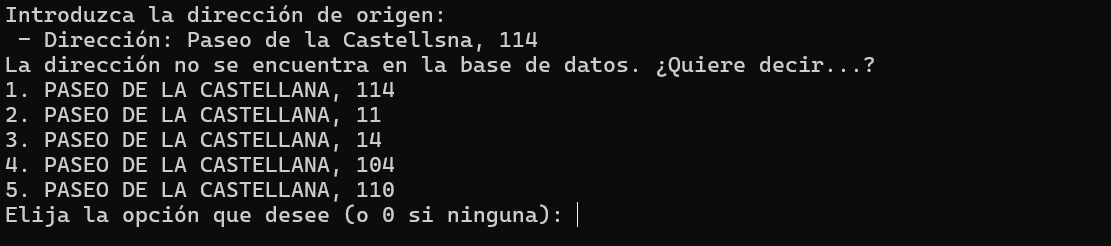
\includegraphics[width=0.85\linewidth]{figs/busqueda_aproximada.png}
\caption{Búsqueda aproximada: la dirección «Paseo de la Castellsna, 114» no existe en el callejero y el programa propone las cinco direcciones más parecidas.}\label{fig:fuzzy}
\end{figure}

\subsection{Grafo de calles}

El grafo de la red viaria de Madrid se obtiene de OpenStreetMap~[5] mediante la librería OSMnx~[2], con la red de vías transitables en coche. La primera ejecución descarga el grafo y lo guarda en un fichero GraphML; las siguientes lo cargan desde dicho fichero.

OSMnx devuelve un multigrafo dirigido (\code{MultiDiGraph}) ya simplificado: los nodos intermedios de una calle se eliminan y solo se conservan intersecciones y extremos, de modo que un mismo tramo puede reunir varios nombres o velocidades en forma de lista. El programa lo transforma en un grafo dirigido simple (\code{DiGraph}): cuando hay aristas paralelas entre dos nodos, se conserva la de menor longitud. Por último, se eliminan los bucles (aristas de un nodo a sí mismo), que no aportan nada a un camino mínimo. Cada nodo guarda sus coordenadas (\code{x} = longitud, \code{y} = latitud) y cada arista, atributos como la longitud en metros (\code{length}), el nombre de la vía (\code{name}), su referencia (\code{ref}), el tipo de vía (\code{highway}) y la velocidad máxima (\code{maxspeed}). La Figura~\ref{fig:grafo} muestra el grafo resultante.

\begin{figure}[H]
\centering
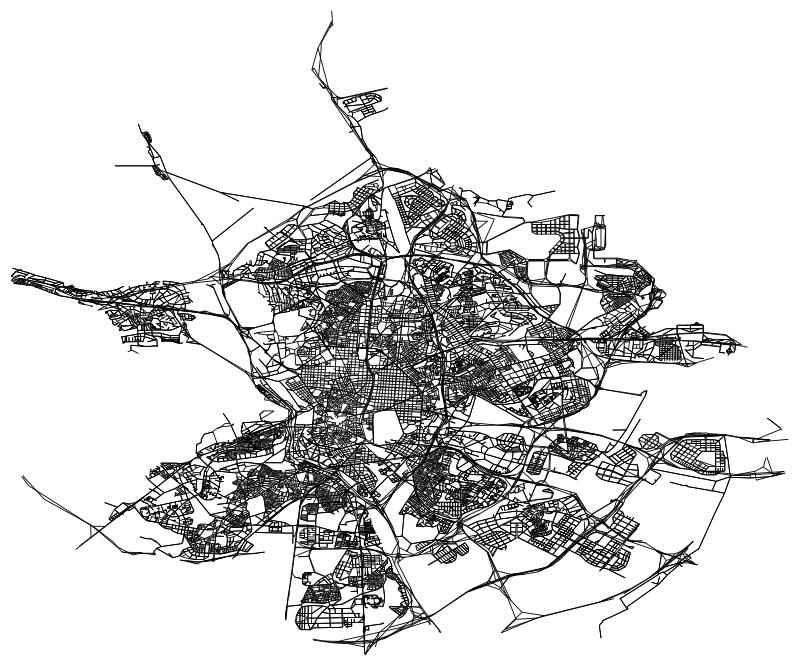
\includegraphics[width=0.78\linewidth]{figs/grafo_madrid.png}
\caption{Grafo de calles de Madrid utilizado por el GPS, dibujado a partir de las coordenadas de sus nodos.}\label{fig:grafo}
\end{figure}

% ---------------- 4 ----------------
\section{Algoritmos sobre grafos pesados}

La biblioteca \code{grafo\_pesado.py} implementa los algoritmos del tema de grafos de la asignatura~[1]. Todas las funciones reciben como parámetro una \emph{función de peso} $w(G,u,v)$ que devuelve el coste de la arista $(u,v)$, lo que permite reutilizarlas con cualquier criterio sin modificar el algoritmo.

\textbf{Dijkstra.} Calcula el árbol de caminos mínimos desde un vértice de origen. Mantiene para cada vértice su distancia provisional, su padre en el árbol y si ya ha sido visitado. En cada iteración extrae de una cola de prioridad (montículo binario del módulo \code{heapq}) el vértice no visitado con menor distancia, lo marca como visitado y relaja sus aristas salientes:
\[
\text{si } \operatorname{dist}(u)+w(u,v)<\operatorname{dist}(v):\quad \operatorname{dist}(v)\leftarrow\operatorname{dist}(u)+w(u,v),\;\; \operatorname{padre}(v)\leftarrow u .
\]
Cuando la distancia de un vértice mejora, se inserta de nuevo en el montículo con la nueva prioridad, y las entradas antiguas se ignoran al extraerlas porque el vértice ya está visitado. El algoritmo es correcto porque todos los pesos son no negativos. Con el montículo, su coste es $O((V+E)\log V)$, frente al $O(V^2)$ de buscar el mínimo recorriendo todos los vértices, lo que resulta imprescindible en un grafo del tamaño del de Madrid.

\textbf{Camino mínimo.} \code{camino\_minimo}, la función que utiliza \code{gps.py}, ejecuta Dijkstra desde el origen y reconstruye el camino recorriendo los padres desde el destino hasta el origen; después invierte la lista. Si el destino no tiene padre en el árbol, no es alcanzable desde el origen (por ejemplo, por calles de sentido único), la función devuelve \code{None} y el programa informa de que no existe una ruta en coche.

\textbf{Prim y Kruskal.} El módulo implementa también estos dos algoritmos, que no intervienen en el cálculo de rutas. Ambos obtienen un árbol abarcador mínimo: un conjunto de aristas que conecta todos los vértices sin formar ciclos y con coste total mínimo. Difieren en su enfoque: el algoritmo de Prim hace crecer el árbol desde un vértice inicial, añadiendo en cada paso la arista más barata que lo conecta con un vértice nuevo, mientras que el de Kruskal recorre las aristas en orden creciente de peso y añade cada una siempre que una dos componentes distintas, es decir, siempre que no genere un ciclo. Es importante no confundir ambos problemas: un árbol abarcador mínimo minimiza el coste total de conectar \emph{todos} los vértices, mientras que un camino mínimo minimiza el coste entre \emph{dos} vértices concretos, que es lo que necesita un GPS.

% ---------------- 5 ----------------
\section{Funciones de peso}

El archivo \code{pesos.py} define las funciones de coste que asignan un valor numérico a cada arista $(u,v)$ del grafo. El usuario elige el criterio de optimización entre las tres opciones de la Tabla~\ref{tab:modos}; en todos los casos, Dijkstra minimiza la suma de los pesos de las aristas del camino.

\begin{table}[H]
\centering
\caption{Modos de cálculo de ruta y funciones de peso asociadas.}\label{tab:modos}
\small
\begin{tabularx}{\linewidth}{@{}>{\raggedright\arraybackslash}p{3.4cm}>{\raggedright\arraybackslash}p{3.4cm}>{\raggedright\arraybackslash}X@{}}
\toprule
\textbf{Modo} & \textbf{Función} & \textbf{Peso de la arista $(u,v)$}\\
\midrule
Más corta (MC) & \code{length\_weight} & $\ell(u,v)$, en metros.\\
Más rápida (MR) & \code{time\_weight} & $t(u,v)=\ell(u,v)/v_{\max}(u,v)$, en segundos.\\
Más rápida con semáforos (MRO) & \code{stoplights\_weight} & $t(u,v)$ más 24 s si $v$ es una intersección.\\
\bottomrule
\end{tabularx}
\end{table}

\subsection{Ruta más corta}

El peso es la longitud física del tramo, $w_{\text{MC}}(u,v)=\ell(u,v)$, tomada del atributo \code{length} de la arista. El camino óptimo es, por tanto, el de menor distancia recorrida.

\subsection{Ruta más rápida}

El peso es el tiempo necesario para recorrer el tramo a la velocidad máxima permitida:
\[
w_{\text{MR}}(u,v)=t(u,v)=\frac{\ell(u,v)}{v_{\max}(u,v)\cdot\frac{1000}{3600}}\quad\text{[s]},
\]
con $\ell$ en metros y $v_{\max}$ en km/h. La velocidad máxima de cada arista se determina así:

\begin{enumerate}
\item Si la arista tiene el atributo \code{maxspeed}, se extrae con una expresión regular el primer número de su valor (los valores de OpenStreetMap pueden incluir texto, como «50 mph» o «ES:urban»). Si el tramo agrupa varias velocidades, se toma la mayor, suponiendo que la vía se rige por la menos restrictiva.
\item Si no tiene \code{maxspeed}, o su valor no contiene ningún número, se asigna una velocidad según el tipo de vía (\code{highway}), de acuerdo con la Tabla~\ref{tab:velocidades}. Si el tramo agrupa varios tipos de vía, se toma la mayor de sus velocidades.
\item Si tampoco el tipo de vía figura en la tabla, se usa un valor por defecto de 30 km/h.
\end{enumerate}

\begin{table}[H]
\centering
\caption{Velocidad asignada según el tipo de vía cuando la arista no indica su velocidad máxima.}\label{tab:velocidades}
\small
\setlength{\tabcolsep}{4pt}\begin{tabular}{@{}lr@{\hspace{1.4em}}lr@{}}
\toprule
\textbf{Tipo de vía} & \textbf{km/h} & \textbf{Tipo de vía} & \textbf{km/h}\\
\midrule
\code{living\_street} & 20 & \code{secondary}, \code{tertiary}, \code{primary} & 50\\
\code{residential} & 30 & \code{trunk}, \code{tertiary\_link}, \code{busway} & 50\\
\code{unclassified} & 40 & \code{motorway\_link} & 70\\
\code{primary\_link}, \code{secondary\_link}, \code{trunk\_link} & 40 & \code{motorway} & 100\\
\bottomrule
\end{tabular}
\end{table}

\subsection{Ruta más rápida con semáforos}

Este modo añade al tiempo de recorrido una penalización por la espera prevista al llegar a una intersección, según el modelo del enunciado:
\[
w_{\text{MRO}}(u,v)=t(u,v)+p(v)\cdot T,\qquad
p(v)=\begin{cases}0{,}8 & \text{si } \deg^-(v)+\deg^+(v)>2,\\ 0 & \text{en otro caso,}\end{cases}\qquad T=30\text{ s}.
\]
La penalización se interpreta como un tiempo esperado: en cada intersección hay un semáforo que se encuentra en rojo con probabilidad 0,8, y en ese caso la espera es de 30 s. Cada intersección añade así $0{,}8\cdot30=24$ s al coste del camino. Se considera intersección todo nodo con más de dos aristas incidentes, contando tanto las entrantes ($\deg^-$) como las salientes ($\deg^+$). Un nodo con dos o menos, como el extremo de una calle sin salida de doble sentido (una arista de entrada y otra de salida), no se penaliza. Como el grafo está simplificado, prácticamente el resto de nodos son cruces entre calles.

La penalización se aplica al nodo de llegada $v$ de cada arista, por lo que un camino de $k$ aristas que atraviesa $n$ intersecciones paga $24n$ segundos además de su tiempo de recorrido. Este modo prefiere, por tanto, vías con pocos cruces aunque sean más largas.

\subsection{Comparación de los tres modos}

La Figura~\ref{fig:modos} muestra la ruta de ejemplo calculada con cada modo. Las tres respuestas son distintas y se explican por la función de peso:

\begin{itemize}
\item \textbf{MC} sigue el eje Castellana--Recoletos--Prado y atraviesa el centro: es la opción más directa. Según las instrucciones de la Figura~\ref{fig:instr}, recorre unos 7,9 km.
\item \textbf{MR} baja por la calle de Serrano, paralela a la Castellana: el criterio ya no es la distancia sino el tiempo, que depende de la velocidad máxima de cada tramo.
\item \textbf{MRO} evita el centro y rodea la ciudad por el este, recorriendo unos 8 km por la Avenida de la Paz (tramo este de la M-30). Aunque la ruta es bastante más larga, la vía tiene muchas menos intersecciones que la trama urbana y una velocidad mayor, de modo que la penalización de 24 s por cruce hace que este rodeo resulte el camino de menor coste.
\end{itemize}

\begin{figure}[H]
\centering
\begin{subfigure}[t]{0.32\linewidth}\centering
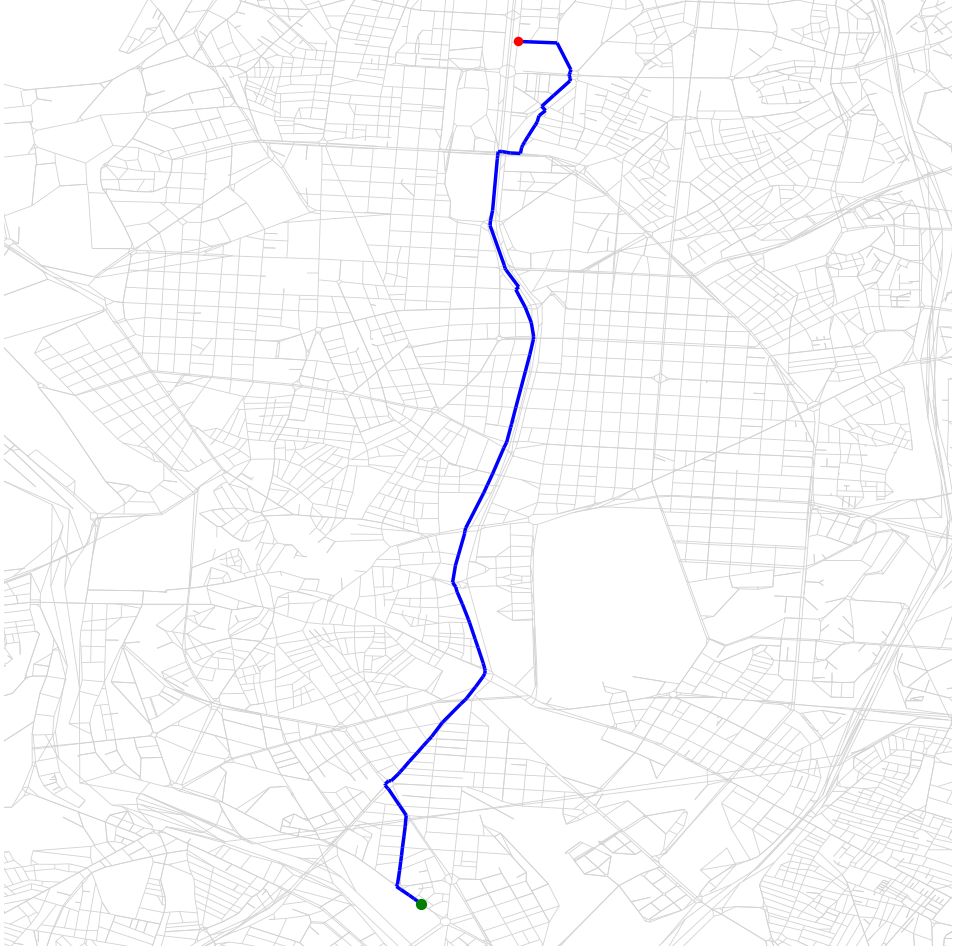
\includegraphics[width=\linewidth]{figs/ruta_mc.png}
\caption{Más corta (MC).}
\end{subfigure}\hfill
\begin{subfigure}[t]{0.32\linewidth}\centering
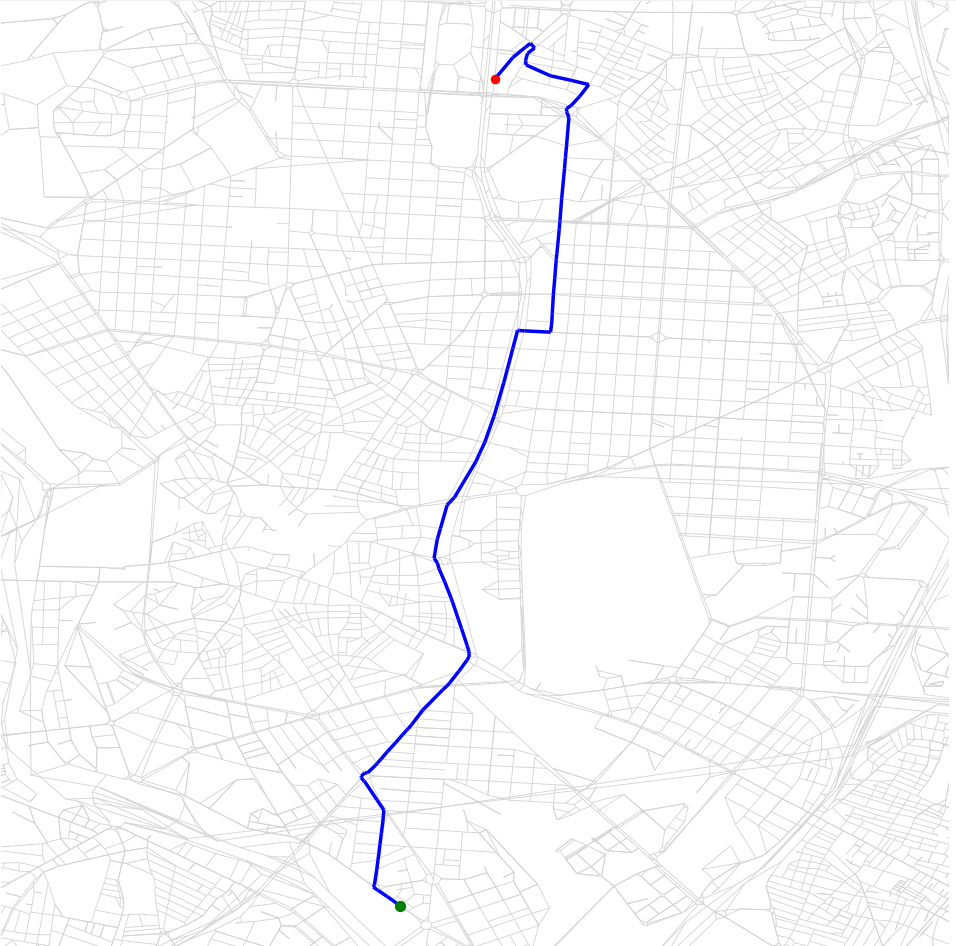
\includegraphics[width=\linewidth]{figs/ruta_mr.png}
\caption{Más rápida (MR).}
\end{subfigure}\hfill
\begin{subfigure}[t]{0.32\linewidth}\centering
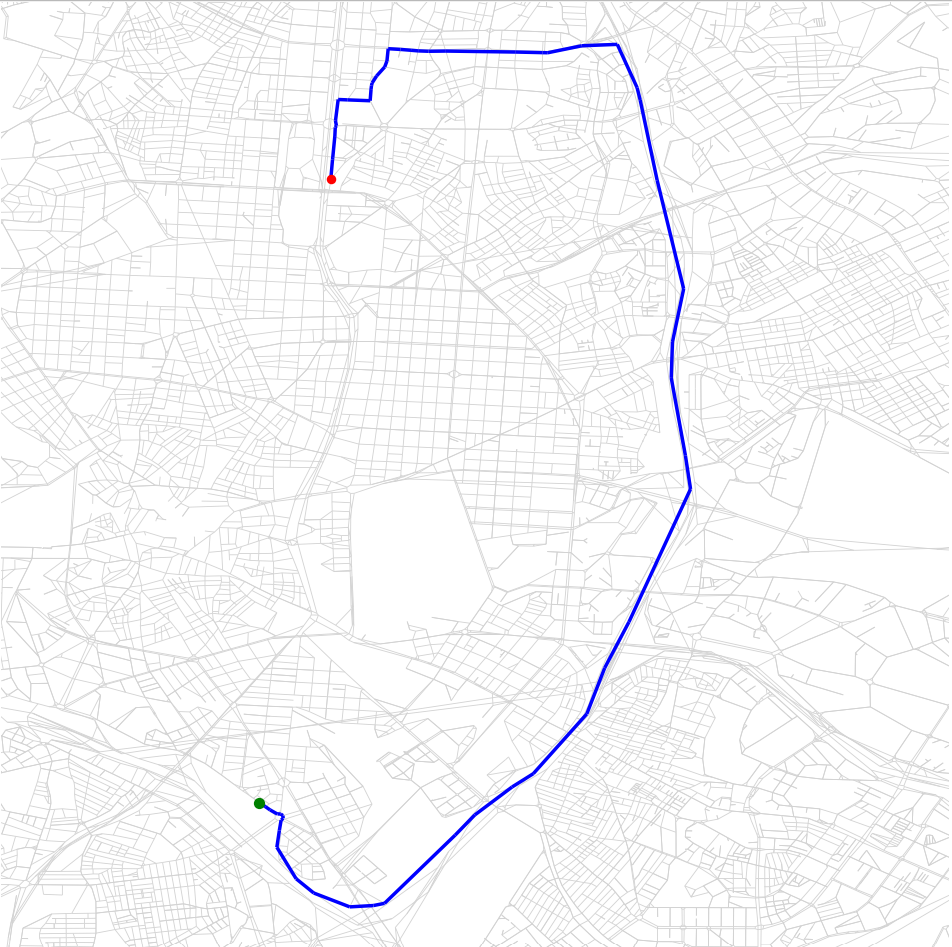
\includegraphics[width=\linewidth]{figs/ruta_mro.png}
\caption{Con semáforos (MRO).}
\end{subfigure}
\caption{Ruta entre el Paseo de la Castellana, 144 (punto rojo) y el Paseo de la Chopera, 14 (punto verde) con cada modo de cálculo. Cada mapa se ajusta a su propia ruta, por lo que la escala no es la misma en los tres.}\label{fig:modos}
\end{figure}

% ---------------- 6 ----------------
\section{Instrucciones de navegación}

A partir de la lista de nodos del camino, el programa genera instrucciones legibles. El proceso tiene tres partes: agrupar los tramos que pertenecen a una misma vía, decidir el tipo de giro en cada cambio de vía y redactar el mensaje correspondiente.

\subsection{Agrupación por vía}

Se recorren las aristas del camino en orden. Para cada arista se obtiene el nombre de la vía: el atributo \code{name} si existe (si el tramo agrupa varios nombres, se unen en la forma «A, B y C»), la referencia \code{ref} si no tiene nombre, o la marca \code{NO-NAME} si no tiene ninguno de los dos. La longitud de cada arista se acumula mientras el nombre se mantiene. Cuando la siguiente arista tiene un nombre distinto, o se llega a la última arista, se emite una instrucción con la distancia acumulada y el contador se reinicia. Así, una calle formada por muchos tramos genera una sola instrucción.

\subsection{Tipo de giro}

En cada cambio de vía se clasifica el giro a partir de los tres nodos implicados: $u$ y $v$, extremos de la última arista de la vía actual, y $w$, final de la primera arista de la nueva vía. Con sus coordenadas se forman los vectores
\[
\mathbf a = v-u = (a_x,a_y),\qquad \mathbf b = w-v = (b_x,b_y),
\]
y se calcula el ángulo entre ellos y la componente $z$ de su producto vectorial:
\[
\theta=\arccos\frac{\mathbf a\cdot\mathbf b}{\lVert\mathbf a\rVert\,\lVert\mathbf b\rVert},\qquad
\mathbf a\times\mathbf b=a_x b_y-a_y b_x .
\]
Si $\theta<30^\circ$, la dirección apenas cambia y se considera que el vehículo sigue recto. En otro caso, el signo del producto vectorial indica el sentido del giro: positivo si $\mathbf b$ queda a la izquierda de $\mathbf a$ (giro antihorario) y negativo si queda a la derecha (Figura~\ref{fig:giro}). Como el redondeo puede dar cocientes ligeramente mayores que 1 en valor absoluto, el coseno se limita al intervalo $[-1,1]$ antes de calcular el arcocoseno.

\begin{figure}[H]
\centering
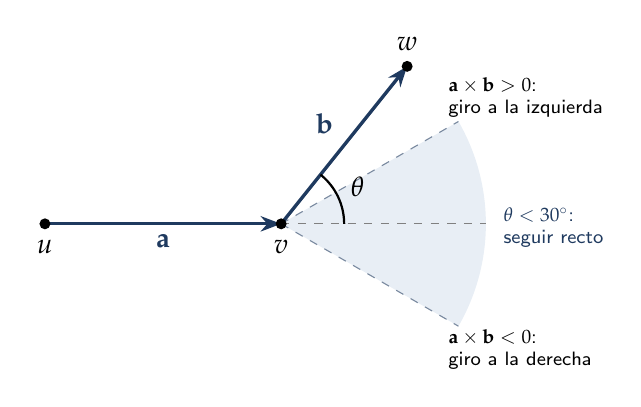
\begin{tikzpicture}[scale=1.0,
  pto/.style={circle,fill=black,inner sep=1.4pt},
  vec/.style={-{Stealth[length=2.6mm]},very thick,azul}]
\coordinate (u) at (0,0);
\coordinate (v) at (3,0);
\coordinate (ext) at (5.6,0);
\coordinate (w) at (4.6,2.0);
% cono de "seguir recto"
\fill[azulclaro] (v) -- ($(v)+(-30:2.6)$) arc[start angle=-30,end angle=30,radius=2.6] -- cycle;
\draw[azul!60,dashed] (v) -- ($(v)+(30:2.6)$);
\draw[azul!60,dashed] (v) -- ($(v)+(-30:2.6)$);
\draw[dashed,gray] (v) -- (ext);
\draw[vec] (u) -- node[below] {$\mathbf a$} (v);
\draw[vec] (v) -- node[above left] {$\mathbf b$} (w);
\pic[draw,thick,"$\theta$",angle eccentricity=1.35,angle radius=0.8cm] {angle=ext--v--w};
\node[pto,label=below:$u$] at (u) {};
\node[pto,label=below:$v$] at (v) {};
\node[pto,label=above:$w$] at (w) {};
\node[font=\sffamily\scriptsize,text=azul,align=left,anchor=west] at ($(v)+(2.7,-0.05)$) {$\theta<30^\circ$:\\ seguir recto};
\node[font=\sffamily\scriptsize,align=left,anchor=west] at (5.0,1.6) {$\mathbf a\times\mathbf b>0$:\\ giro a la izquierda};
\node[font=\sffamily\scriptsize,align=left,anchor=west] at (5.0,-1.6) {$\mathbf a\times\mathbf b<0$:\\ giro a la derecha};
\end{tikzpicture}
\caption{Clasificación del giro en el nodo $v$. Si $\mathbf b$ cae dentro de la zona sombreada ($\theta<30^\circ$) se sigue recto; fuera de ella, el signo de $\mathbf a\times\mathbf b$ distingue la izquierda de la derecha. En el ejemplo, $\theta\approx51^\circ$ y el producto vectorial es positivo: giro a la izquierda.}\label{fig:giro}
\end{figure}

\subsection{Redacción de los mensajes}

Con el nombre de la vía actual, el de la siguiente y el tipo de giro, el mensaje se elige según los casos de la Tabla~\ref{tab:mensajes}. Las calles sin nombre se tratan aparte porque no se puede decir «por» qué vía se avanza; en ese caso la distancia y la maniobra se combinan en un único mensaje.

\begin{table}[H]
\centering
\caption{Mensajes generados en cada caso ($X$: distancia acumulada; $N_1$: vía actual; $N_2$: vía siguiente).}\label{tab:mensajes}
\small
\begin{tabularx}{\linewidth}{@{}>{\raggedright\arraybackslash}p{3.1cm}>{\raggedright\arraybackslash}p{3.2cm}>{\raggedright\arraybackslash}X@{}}
\toprule
\textbf{Vía actual} & \textbf{Situación} & \textbf{Mensaje}\\
\midrule
Con nombre & Último tramo & «Avance $X$ m por $N_1$ hasta llegar a su destino.»\\
 & Giro a izquierda o derecha & «Avance $X$ m por $N_1$.» y «Gire a la izquierda/derecha hacia $N_2$.» (sin «hacia $N_2$» si la vía siguiente no tiene nombre)\\
 & Cambio de vía en recto & «Avance $X$ m por $N_1$.» y «Siga recto hacia $N_2$.» (este último solo si la vía siguiente tiene nombre)\\
\midrule
Sin nombre & Último tramo & «Avance $X$ m hasta llegar a su destino.»\\
 & Giro a izquierda o derecha & «Avance $X$ m y gire a la izquierda/derecha hacia $N_2$.»\\
 & Cambio de vía en recto & «Siga recto $X$ m hasta $N_2$.»\\
\bottomrule
\end{tabularx}
\end{table}

La Figura~\ref{fig:instr} muestra las instrucciones de la ruta de ejemplo en modo MC. Se aprecia la agrupación: los 2,4 km de la Castellana aparecen en dos instrucciones, separadas solo por el paso por la Plaza del Doctor Marañón, que en OpenStreetMap es una vía distinta. Lo mismo ocurre en las plazas de Colón y del Emperador Carlos V, que se atraviesan en recto.

\begin{figure}[H]
\centering
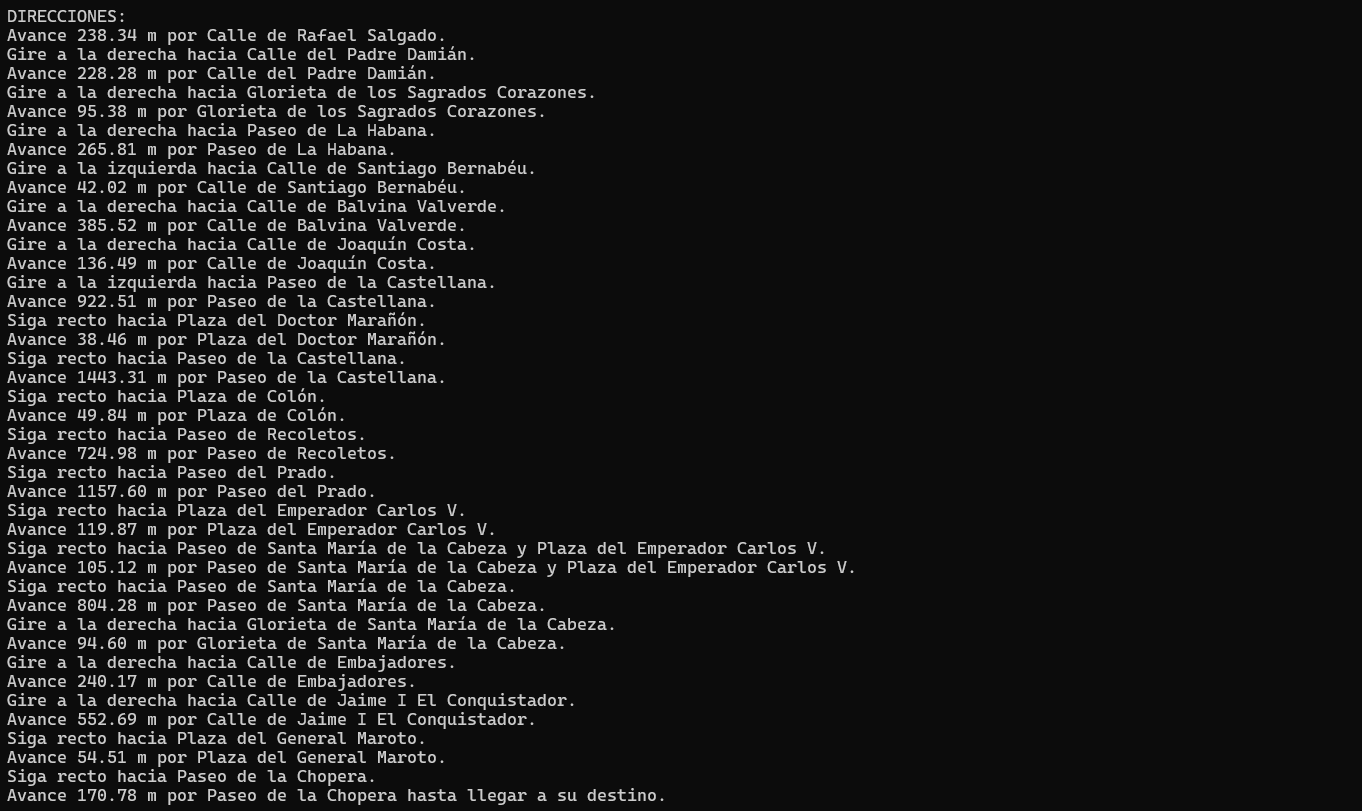
\includegraphics[width=\linewidth]{figs/instrucciones_mc.png}
\caption{Instrucciones de navegación generadas para la ruta de ejemplo en modo MC.}\label{fig:instr}
\end{figure}

% ---------------- 7 ----------------
\section{Representación gráfica de la ruta}

Para facilitar la interpretación de la ruta, se dibuja el grafo de calles con las funciones de NetworkX y Matplotlib, usando como posición de cada nodo sus coordenadas, y se resalta el camino obtenido en azul, con el origen en rojo y el destino en verde. Para ampliar la zona de interés, se calcula el recuadro mínimo que contiene todos los nodos del trayecto, se convierte en un cuadrado centrado en él con un 10\,\% de margen y se ajustan los límites de los ejes a ese cuadrado, manteniendo la relación de aspecto 1:1. Los mapas de la Figura~\ref{fig:modos} son el resultado de esta función.

% ---------------- 8 ----------------
\section{Limitaciones}

\begin{itemize}
\item El modelo de semáforos es el del enunciado: penaliza por igual todas las intersecciones, tengan o no semáforo, y no tiene en cuenta el tráfico real.
\item El ángulo de giro se calcula directamente sobre longitud y latitud. A la latitud de Madrid, un grado de longitud mide unas tres cuartas partes de un grado de latitud, por lo que los ángulos se deforman ligeramente; para clasificar giros con un umbral de 30° el efecto es pequeño.
\item El giro se evalúa solo con los tramos inmediatamente anterior y posterior al cambio de vía, y solo se anuncian las maniobras en los cambios de nombre: una curva pronunciada dentro de una misma calle no genera instrucción.
\item La búsqueda aproximada compara la entrada con todas las direcciones del callejero, por lo que es más lenta que la búsqueda exacta; solo se ejecuta cuando esta falla.
\end{itemize}

% ---------------- 9 ----------------
\section{Uso de herramientas de inteligencia artificial}

Durante la elaboración de la práctica se utilizaron herramientas de inteligencia artificial con los siguientes fines: pulir el código, corregir errores y resolver dudas puntuales. En particular, sirvieron de apoyo para utilizar las librerías de grafos, corregir pequeños errores del código y aclarar dudas sobre los algoritmos de Prim, Kruskal y Dijkstra. Su papel fue exclusivamente de apoyo: todo el trabajo entregado fue realizado por los integrantes del grupo.

% ---------------- Referencias ----------------
\Needspace{10\baselineskip}
\section*{Referencias}
\addcontentsline{toc}{section}{Referencias}
\begin{enumerate}[label={[\arabic*]},leftmargin=2.2em]
\item Matemática Discreta, \emph{Transparencias del Tema 6}. Universidad Pontificia Comillas (ICAI).
\item G. Boeing. \emph{OSMnx documentation}. \url{https://osmnx.readthedocs.io}
\item NetworkX developers. \emph{Tutorial — NetworkX documentation}. \url{https://networkx.org/documentation/stable/tutorial.html}
\item Ayuntamiento de Madrid. \emph{Callejero oficial del Ayuntamiento de Madrid: relación de direcciones vigentes, con coordenadas}. Portal de Datos Abiertos, licencia CC BY 4.0. \url{https://datos.madrid.es}
\item OpenStreetMap contributors. \emph{OpenStreetMap}, datos bajo licencia ODbL. \url{https://www.openstreetmap.org}
\end{enumerate}

\end{document}
